% !TEX encoding = UTF-8
% !TEX TS-program = pdflatex
% !TEX root = ../tesi.tex

%**************************************************************
\chapter{Introduzione}
\label{cap:introduzione}
%**************************************************************

%Introduzione al contesto applicativo.\bigskip

\intro{Sarà mostrata nel presente capitolo una panoramica sull'azienda ospitante, Sync Lab e descritte alcune norme tipografiche che saranno usate nel corso del documento.}

%**************************************************************

\section{Convenzioni tipografiche}

% \begin{description}
% \item[{\hyperref[cap:processi-metodologie]{Il secondo capitolo}}] descrive ...

% \item[{\hyperref[cap:descrizione-stage]{Il terzo capitolo}}] approfondisce ...

% \item[{\hyperref[cap:analisi-requisiti]{Il quarto capitolo}}] approfondisce ...

% \item[{\hyperref[cap:progettazione-codifica]{Il quinto capitolo}}] approfondisce ...

% \item[{\hyperref[cap:verifica-validazione]{Il sesto capitolo}}] approfondisce ...

% \item[{\hyperref[cap:conclusioni]{Nel settimo capitolo}}] descrive ...
% \end{description}

Riguardo la stesura del testo, relativamente al documento sono state adottate le seguenti convenzioni tipografiche:
\begin{itemize}
	\item Gli acronimi, le abbreviazioni e i termini ambigui o di uso non comune menzionati vengono definiti nel glossario, situato alla fine del presente documento;
	\item Per la prima occorrenza dei termini riportati nel glossario viene utilizzata la seguente nomenclatura: \gls{api}\gloss. Le successive, avranno esclusivamente il colore celeste.
	\item I termini in lingua straniera di uso non comune o facenti parte del gergo tecnico sono evidenziati con il carattere \emph{corsivo}.
\end{itemize}

%**************************************************************

\section{L'azienda}

\begin{figure}[H]
	\centering
	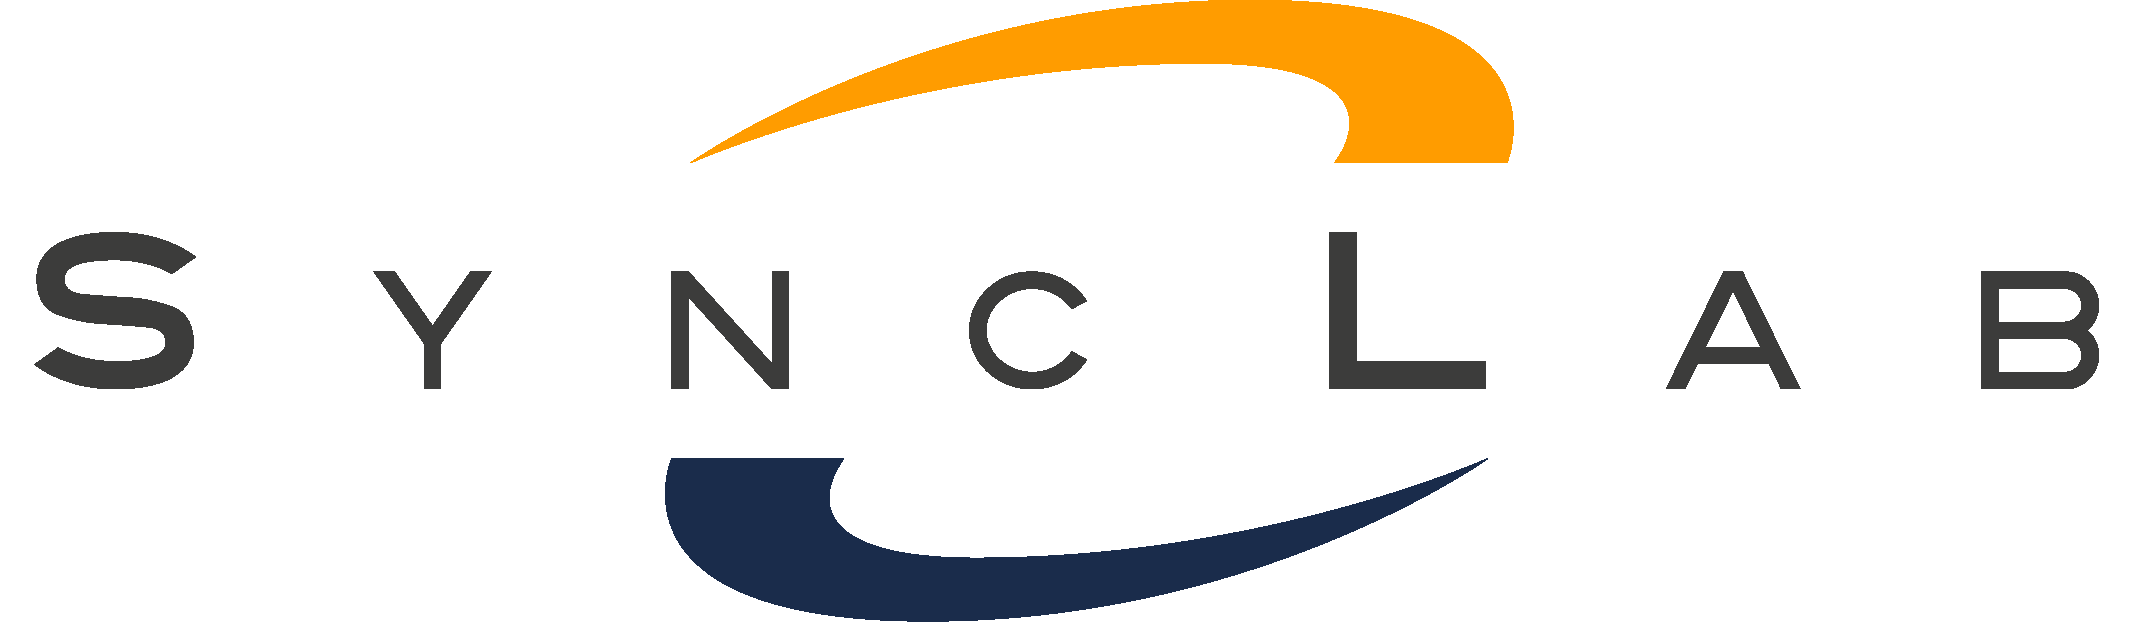
\includegraphics[width=\textwidth/2]{immagini/logo-synclab.png}
	\caption{Logo Sync Lab}
\end{figure}

\subsection{Profilo aziendale}
\myCompany\ è una società di consulenza informatica fondata nel 2002 con sedi a Napoli, Roma, Milano e Padova.

Fin dai primi anni Sync Lab è rapidamente cresciuta nel mercato \gls{ict}, consolidando i rapporti con clienti e partner, raggiungendo un organico aziendale di oltre 200 risorse,
una solida base finanziaria e una diffusione sul territorio attraverso le sue quattro sedi.

L'organico aziendale è andato crescendo in modo continuo e rapido, in relazione
all'apertura delle varie sedi ed alla progressiva crescita delle stesse.

La grande attenzione alla gestione delle risorse umane ha fatto di Sync Lab un
riferimento in positivo per quanti volessero avviare o far evolvere in chiave professionale la propria carriera.

Il basso \textit{turn-over} testimonia la voglia dei collaboratori di condividere il progetto comune, assumendo all'interno di esso ruoli e responsabilità che solo un processo
evolutivo così intenso può offrire.
I ricavi hanno avuto un incremento proporzionale alla crescita dell'azienda beneficiando dell'approccio adattativo e diversificato al mercato.

\subsection{Servizi}

\myCompany\ è un'azienda leader nella consulenza tecnologica, impegnata in un
processo continuo di identificazione e messa in opera di soluzioni per i clienti finalizzate
alla creazione di valore.

L'azienda supporta le esigenze di innovazione di tutte le
organizzazioni ed in ogni settore di mercato nell'ambito \gls{it}, con
servizi in ambito:
\begin{itemize}
	\item \textit{Business Consultancy};
	\item \textit{Project Financing};
	\item \textit{IT Consultancy};
\end{itemize}

Sync Lab ha come punti di forza la qualità dei servizi offerti (certificazioni \acrshort{iso}\gloss\ 9001,
ISO 14001, ISO 27001, \acrshort{ohsas} 18001) ed un'accurata gestione delle risorse umane.
L'approfondita conoscenza di processi e tecnologie, maturata in esperienze altamente
significative e qualificanti, fornisce l'\textit{expertise} e il \textit{know-how} necessari per gestire
progetti di elevata complessità, dominando l'intero ciclo di vita: Studio di fattibilità,
Progettazione, Implementazione, \textit{Governance} e \textit{Post Delivery}.

L'offerta di consulenza specialistica trova le punte di eccellenza nella progettazione di
architetture software avanzate, siano esse per applicativi di dominio, per sistemi di
\gls{bss}, per sistemi di integrazione (\acrshort{eai}/\acrshort{soa}) o per sistemi di
monitoraggio applicativo/territoriale.

Il laboratorio RD (Ricerca e Sviluppo) dell'azienda è sempre al passo con i nuovi
paradigmi tecnologici e di comunicazione, ad esempio \gls{big-data}\gloss, \gls{cloud-computing}\gloss,
\gls{iot}\gloss, Mobile e Sicurezza \acrshort{it}, per supportare i propri clienti nella creazione
ed integrazione di applicazioni, processi e dispositivi.

Le attività in ambito \textit{Educational} ed RD hanno permesso di acquisire una profonda
conoscenza degli strumenti di finanza agevolata fruendone direttamente ed interagendo
con enti di supporto ai progetti innovativi dei propri clienti. L'azienda, grazie alla rete
di relazioni a livello nazionale ed internazionale, ha ottenuto importanti finanziamenti
in progetti RD europei (FP7 e H2020).

\subsection{Settori d'impiego}

Sync Lab si sta sempre più specializzando in vari settori d'impiego: dal mondo \textit{banking}
all'\textit{assurance} con una nicchia importante nell'ambito sanità in cui vanta un prodotto
d'eccellenza per la gestione delle cliniche private.
L'azienda inoltre ha recentemente fondato una collegata \textit{Sync Security} che si occupa
espressamente del mondo della \textit{cyber security} e sicurezza informatica in generale.

%**************************************************************
